\documentclass{article}
%\usepackage[french]{babel}
\usepackage[utf8]{inputenc}
\usepackage[justification=centering]{caption} % pour centrer le texte des légendes qui sont sur plusieurs lignes
%\documentclass[a4paper,10pt]{scrartcl}


\title{Compte-rendu du projet Phare - CDFR 2020}
\author{Gabriel-Robez Baptiste, Equipe Phare}
\date{05/12/19}

\pdfinfo{%
  /Title    (Compte-rendu du projet Phare - CDFR 2020)
  /Author   (Gabriel-Robez Baptiste, Equipe Phare)
  /Subject  (Phare)
  /Keywords (Phare, Robotronik)
}
\usepackage[utf8]{inputenc}
\usepackage{graphicx}
\usepackage[top=2cm, bottom=3cm, left=2.5cm, right=2.5cm]{geometry}



\begin{document}
\maketitle

Mission : Déployer le phare et illuminer l'océan pour que les bateaux puissent rentrer au port en toute
sécurité.

\section{Caractéristiques du phare}

Le phare est une structure immobile mais déployable sur le jeu. Elle se situe sur la zone rocheuse, à l'arrière
de la table de jeu, du même côté que la zone de départ de l'équipe.

\subsection{Contraintes}

\begin{itemize}
\item Le phare ne peut pas être activé par un élément externe à la table de jeu (membre de l’équipe, télécommande
 depuis le public, etc.). Un phare est considéré comme activé s’il a notablement changé de forme
ou d’aspect par rapport au début du match.
\item Le phare peut uniquement être activé pendant le match et au contact d’un des robots de l’équipe.
\item Le déclenchement du phare doit se faire au moment du contact, mais le mode d’activation peut être
effectuée par tout moyen, y compris sans fil.
\item A aucun moment la projection verticale du phare ne doit depasser les limites de la zone rocheuse.
\item En conséquence, le phare aura les contraintes dimensionnelles suivantes :
    \begin{itemize}
    \item Profondeur maximum : 222 mm
    \item Largeur maximum : 450 mm
    \item Hauteur initiale maximum : 300 mm
    \item Hauteur minimum de la source lumineuse (déployée) : 700 mm
    \item Hauteur déployée maximum : 900 mm
    \end{itemize}
\item Le poids du phare ne doit pas excéder 3 kg.
\item Le phare doit avoir un déploiement en hauteur pendant le déroulement du match. Ce déploiement ne
peut avoir lieu qu’après l’activation du phare.
\item Le plan horizontal de la zone rocheuse est percé d’une rainure de 10 mm de large allant du centre du
support au milieu du côté arrière. Cette rainure doit être utilisée pour sécuriser le phare sur la zone
rocheuse grâce à l’utilisation d’une tige filetée de diamètre 8 mm et d’un écrou papillon.
\item Le phare doit rester allumé et déployé même après la fin du match.
\item Le phare pourra contenir une source d’alimentation électrique. Le cas échéant, un bouton d’arrêt d’urgence
 (conforme aux mêmes spécifications que celles des boutons d’arrêt d’urgence des robots) coupant
directement l’alimentation doit équiper le phare. Celui-ci doit être bien visible, facilement accessible et
devra rester à une hauteur constante. Le phare pourra être alimentée avant le début du match sans
toutefois être activé.
\item L’action ne doit pas être dangereuse pour le public, les personnes autour de la table, l’aire de jeu ou les
robots.
\item Le phare peut comporter un écran mais il est seulement autorisé d’y afficher des informations relatives
au match en cours. Il ne devra pas afficher de vidéos, images, photos ou publicités.
\item Une fois allumée, la lumière du phare doit être visible depuis le public, mais ne doit éblouir personne.
\item La lumière du phare devra effectuer un mouvement de balayage apparent ou physique de la source
lumineuse ; le déplacement d’un masque devant la source est autorisé. Le balayage doit être visible par
le public sur au moins 180 degrés de rotation par rapport au devant de la table.
\end{itemize}

\begin{figure}[!h]
\centering
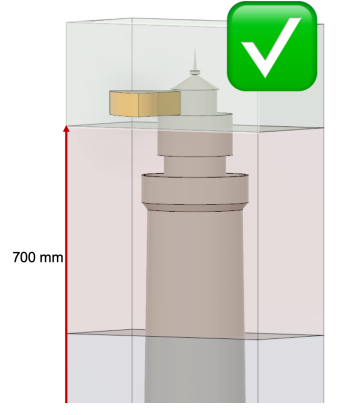
\includegraphics[scale=0.7]{Pictures/deploiement.png}
\caption{Déploiement du phare}
\end{figure}

\begin{figure}[!h]
\centering
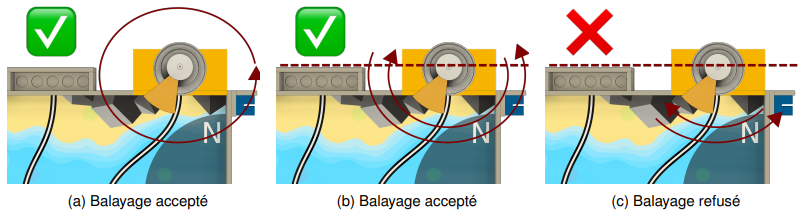
\includegraphics[scale=0.7]{Pictures/eclairage.png}
\caption{Contraintes sur l'éclairage}
\end{figure}

\pagebreak

\subsection{Points}
\begin{itemize}
\item 2 points pour avoir déposé le phare sur la zone zone rocheuse avant le début match ;
\item 3 points supplémentaires pour avoir activé le phare durant le match ;
\item 10 points supplémentaires si le phare est correctement déployé et allumé avant la fin du match.
\end{itemize}


\section{Stratégie adoptée}
Le phare sera composé de trois étages. Le système lumineux se trouvera au sommet du 3ème étage. \\
Le mécanisme permettant le déploiement sera un système à crémaillère et roue crantée,
car il garantit une bonne stabilité et plus facile à mettre en mouvement par des moteurs électriques. \\
Avant le déploiement, les trois étages sont imbriqués les uns dans les autres, et disposés autour de la
batterie et du microcontrôleur, au centre du 1er étage. \\
\begin{figure}[!h]
\centering
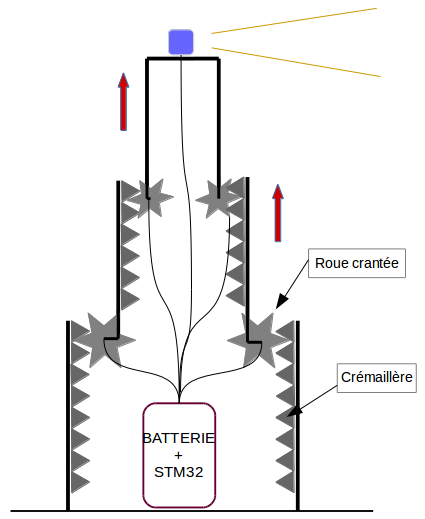
\includegraphics[scale=0.7]{Pictures/Schema_phare.png}
\caption{Vue transversale du phare}
\end{figure}

\pagebreak

Aux étages 1 et 2, deux crémaillères seront disposées verticalement et se feront face (donc un total de 4
crémaillères). Sur les deux faces restantes, des glissières seront disposées verticalement pour guider les
étages dans leur translation (donc un total de 4 glissières). Le troisième étage ne comporte ni crémaillère,
ni glissière.


\begin{figure}[!h]
\centering
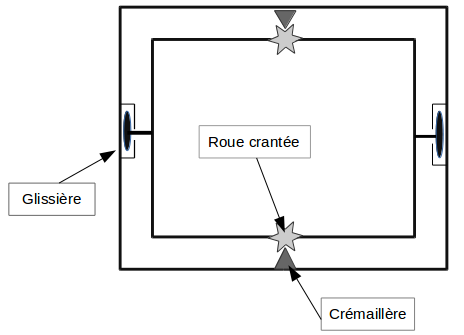
\includegraphics[scale=0.7]{Pictures/Schema_phare2.png}
\caption{Vue en coupe, de dessus, du phare}
\end{figure}


\end{document}
